\chapter{Przeprowadzone badania}\label{WykonaneBadania}
Głównym celem niniejszej pracy były badania wpływu wybranych funkcji sąsiedztwa na możliwość późniejszego wykorzystania sieci samoorganizujących w zadaniach klasyfikacji danych. Do przeprowadzenia badań wykorzystano implementację opisaną w rozdziale \ref{Opis_rozwiazania}. 
\\Badania przeprowadzono na trzech popularnych zbiorach uczących: "MNIST" \cite{MNIST}, "IRIS" \cite{IRIS} i \\Cardiotocography\cite{Patologie}. Każdy z tych zbiorów danych zostanie szczegółowo opisany w osobnej sekcji prezentowanego rozdziału.

W badaniach skupiono się na analizie wpływu wybranej funkcji sąsiedztwa na wartość błędu kwantyzacji, błędu topograficznego i na ocenie jakości klasteryzacji danych na podstawie uzyskanych map zwycięzców. Porównano również dwie rozbieżne kwestie podnoszone w literaturze – dotyczące natury promienia w sieciach SOM. Rozważano, czy promienie sąsiedztwa powinny przyjmować wyłącznie wartości całkowite, tak jak opisano to w pozycji \cite{Kohonen}, czy też mogą być liczbami niecałkowitymi, tak jak przedstawiono to w \cite{Haykin}. Porównania dokonano dla dwóch topologii sieci - prostokątnej z ośmioma sąsiadami i heksagonalnej. 

W celu realizacji postawionych założeń przyjęto jednolitą metodologię badań, opisaną w sekcji \ref{metodologiaBadań}.

\section{Metodologia badań}\label{metodologiaBadań}

Procedura wykonywania badań była jednakowa dla każdego zbioru uczącego. Początkowym etapem było wczytanie danych do programu i wstępne ich przetworzenie. Na tym etapie zbiór danych dzielony był na zbiór uczący i zbiór testowy, w proporcjach osiemdziesiąt (80) do dwudziestu (20) procent. Wyjątkiem tutaj były badanie na zbiorze IRIS, co uzasadniono w sekcji \ref{Irys_sekcja}. Następnie wszystkie dane były normalizowane, do zakresu od zera do jeden. Normalizacja przebiegała według wzoru \ref{normalizacja}.
\begin{equation} \label{normalizacja}
z' = a_g + \frac{(z - z_{\text{min}})}{(z_{\text{max}} - z_{\text{min}})} \cdot (b_g - a_g),
\end{equation}
gdzie \( z \) oznacza oryginalną wartość w zbiorze danych, \( z' \) to przeskalowana wartość, \( z_{\text{min}} \) i \( z_{\text{max}} \) reprezentują odpowiednio minimalną i maksymalną wartość w kolumnie danych, zaś \( a_g \) i \( b_g \) to granice przedziału skalowania ( \( a_g = 0 \) oraz \( b_g = 1 \)).

Liczba epok oraz parametry sieci były dostosowywane indywidualnie dla każdego zbioru uczącego, zgodnie z zasadami zaprezentowanymi w sekcji \ref{Zasady_doboru_parametrow}. Wartości tych parametrów pozostawały takie same dla wszystkich funkcji sąsiedztwa użytych przy treningu i ewaluacji modeli. Również funkcje zmiany współczynnika uczenia i zasięgu sąsiedztwa były jednolite w obrębie każdego zbioru uczącego. Pewną stałą wśród wszystkich badań była zastosowana miara odległości między wzorcami wejściowymi, a wektorami wag. Użyto miary euklidesowej, opisanej w sekcji \ref{eq:euklidesowa}, ze względu na jej popularność w innych pracach \cite{Kohonen,breast,Marine_Traffic}.

Ewaluacja modeli polegała na wyznaczeniu wartości średniego błędu kwantyzacji oraz błędu topograficznego, na danych testowych, dla każdego modelu, stworzonego z zastosowaniem innej funkcji sąsiedztwa w procesie uczenia. Tworzone były również mapy zwycięzców do wizualnej oceny jakości klasteryzacji.

W kolejnych sekcjach rozdziału zaprezentowano osiągnięte rezultaty. W każdej z sekcji \ref{Irys_sekcja}, \ref{Patologie_sekcja} oraz \ref{MNIST_sekcja} opisano wykorzystany zbiór uczący wraz z uzasadnieniem wyboru. Umieszczono w nich także tabele z porównaniem wartości średnich błędów kwantyzacji i topograficznego oraz mapę zwycięzców dla modelu z najmniejszym wynikami obu błędów. Zdecydowano się na prezentację tylko jednej z map zwycięzców, z uwagi na ilość wytrenowanych modeli.

%IRYSY SEKCJA

\section{Badania na zbiorze IRIS}\label{Irys_sekcja}
Zbiór danych \textit{Iris} jest jednym z najpopularniejszych zbiorów danych wykorzystywanych w zadaniach klasyfikacji i klasteryzacji. Przez swoją prostą strukturę, umożliwia wstępne zbadanie wszelkiego rodzaju algorytmów analizy danych, dlatego jest częstym przedmiotem badań \cite{IRIS}. Zbiór ten powstał w 1936 roku i zawiera 150 próbek opisujących 3 gatunki  irysów (roślina ozdobna). Każdy wektor danych zawiera cztery cechy opisujące morfologię kwiatu tej rośliny: długość działki kielicha (\textit{sepal length}), szerokość działki kielicha (\textit{sepal width}), długość płatka (\textit{petal length}) oraz szerokość płatka (\textit{petal width}).
\\Dane wejściowe podzielone są na 3 klasy, reprezentujące różne gatunki rośliny:
\begin{itemize}
\item \textbf{Setosa}:  50 próbek, z etykietą "0",
\item \textbf{Versicolor}:  50 próbek, z etykietą "1"
\item \textbf{Virginica}:  50 próbek, z etykietą "2".
\end{itemize}

Zbiór danych wydaje się z pozoru prosty do klasyfikacji, ze względu na swoją wielkość i ograniczoną liczbę cech. Problemy może jednak sprawiać specyficzny podział na klasy, występujący w tym zbiorze. Wynika to z faktu, że irysy z gatunku \textbf{Versicolor} mają podobną budowę morfologiczną, jak irysy z gatunku \textbf{Virginica}. 
Prowadzi to często do trudności w jednoznacznej klasyfikacji tych roślin.

Zbiór danych został wybrany z uwagi na niewielki rozmiar, równą liczność klas oraz ograniczoną liczbę cech. W badaniu skupiono się na ocenie działania sieci samoorganizującej się w takim zbiorze, a także na analizie jej zdolności do zachowania topologii danych. Zakłada się, że taka właściwość sieci SOM powinna prowadzić do wyraźnego oddzielenia danych należących do klasy \textit{Setosa} od pozostałych, natomiast dane z klas \textit{Versicolor} i \textit{Virginica}, ze względu na ich podobieństwo, mogą częściowo się nakładać na mapie zwycięzców.

Do tworzenia modeli wykorzystano siatkę 8 na 8 neuronów, z początkowym promieniem równym 4 i początkową wartością współczynnika uczenia równą 0.3. Wykorzystano funkcję liniową, opisaną w sekcji \ref{eq:linear_decay}, dla zmiany wartości promienia  oraz funkcję wymierną, opisaną w sekcji \ref{eq:exponential_decay},  dla zmiany wartości współczynnika uczenia. Ze względu na ograniczoną liczbę danych w zbiorze, każda z sieci była trenowane przez 10000 epok.

W przypadku tego (dość małego zbioru) zbioru, dane nie były dzielone na zbiór uczący i testowy. Skutkowało to ewaluacją modeli na tych samych danych, na których przeprowadzone zostało uczenie sieci. Sieć Kohonena potraktowano tutaj jako narzędzie do analizy i klasyfikacji danych wyłącznie w obrębie zbioru uczącego. Takie zastosowanie sieci jest również popularne, między innymi w pozycji \cite{breast}.

Tabela \ref{IRIS_tabela} przedstawia otrzymane wartości błędów kwantyzacji i topograficznych. Zastosowane skróty oznaczają kolejno: \(\textbf{hex}_{ncp}\) – badania dla topologii heksagonalnej i niecałkowitych wartości promienia, \(\textbf{rect}_{ncp}\) – badania dla topologii prostokątnej z ośmioma sąsiadami i niecałkowitych wartości promienia, \(\textbf{hex}_{cp}\) – badania dla topologii heksagonalnej i całkowitych wartości promienia, oraz \(\textbf{rect}_{cp}\) – badania dla topologii prostokątnej z ośmioma sąsiadami i całkowitych wartości promienia.
\begin{table}[h]
\centering
\caption{Wartości błędów topograficznych i kwantyzacji  z testów na zbiorze IRIS}
\label{IRIS_tabela}
\begin{tabular}{|l|l|l|l|l|l|}
\hline
\textbf{\begin{tabular}[c]{@{}l@{}}funkcja\\ sasiedztwa\end{tabular}} & \textbf{Rodzaj błędu} & \(\textbf{hex}_{ncp}\) & \(\textbf{rect}_{ncp}\) & \(\textbf{hex}_{cp}\) & \(\textbf{rect}_{cp}\) \\ \hline
\multirow{2}{*}{\textbf{Gaussa}}                                      & błąd kwantyzacji      & 0.0837                 & 0.0946                  & 0.0931                & 0.0936                 \\ \cline{2-2}
                                                                      & błąd topograficzny    & 0.0063                & 0.1128                  & 0.0338                & 0.0902                 \\ \hline
\multirow{2}{*}{\textbf{trójkątna}}                                   & błąd kwantyzacji      & 0.0630                 & 0.0626                  & 0.0574                & 0.0576                 \\ \cline{2-2}
                                                                      & błąd topograficzny    & 0.0812                 & 0.2066                  & 0.1123                & 0.2130                 \\ \hline
\multirow{2}{*}{\textbf{prostokątna}}                                     & błąd kwantyzacji      & 0.0942                 & 0.0805                  & 0.0858                & 0.0769                 \\ \cline{2-2}
                                                                      & błąd topograficzny    & 0.0096                 & 0.1153                  & 0.0420                & 0.1430                 \\ \hline
\multirow{2}{*}{\textbf{eksponencjalna}}                              & błąd kwantyzacji      & 0.0810                 & 0.0769                  & 0.0820                & 0.0741                 \\ \cline{2-2}
                                                                      & błąd topograficzny    & 0.0600                 & 0.1133                  & 0.0661                & 0.1532                 \\ \hline
\end{tabular}
\end{table}

\subsection{Wnioski z badań na zbiorze IRIS}
Maksymalny błąd kwantyzacji dla tego zbioru danych, zdefiniowany zależnością \ref{maksymalny_blad_kwantyzacji} przyjmuje wartość\(\sqrt{4} =2\). Najlepszą z uzyskanych wartości w przypadku tego błędu, wynosi 0.0574 i stanowi \(2.87\%\) wartości maksymalnej. Otrzymano ją  dla zastosowania funkcji trójkątnej, z promieniem sąsiedztwa zmieniającym się w sposób całkowity oraz topologią heksagonalną. W tym wypadku wystąpił jednak  znaczny błąd topograficzny, co przeniosło się bezpośrednio na rozkład klas na mapie zwycięzców. Podobnie, przy innych sieciach trenowanych za pomocą tej funkcji osiągnięto wysokie błędy topograficzne, które uniemożliwiają skuteczne stosowanie zaproponowanej funkcji trójkątnej w tym przypadku. Otrzymane rezultaty mogą wynikać z postaci funkcji trójkątnej stosowanej w zaproponowanej implementacji.
Szersze skomentowanie wyników błędów otrzymanych przy trenowaniu sieci z użyciem funkcji trójkątnej przedstawiono w rozdziale \ref{Podsumowanie_badań}.

Użycie funkcji eksponencjalnej pozwoliło na zmniejszenie wartości błędów topograficznych, w stosunku do ich wartości w przypadku stosowania funkcji trójkątnej. 
Zadowalające rezultaty osiągnięto także przy zastosowaniu funkcji progowej. W każdej możliwej kombinacji topologia - sposób zmiany promienia, osiągnięto rezultaty nieznacznie gorsze od funkcji Gaussa. Jest to dość nieoczekiwana obserwacja, która może sugerować, że dla prostych zbiorów danych stosowanie funkcji progowej jest warte rozważenia.

Najmniejsze wartości błędu kwantyzacji i topograficznego, wraz z najlepszymi rezultatami na mapie zwycięzców, osiągnięto przy stosowaniu funkcji Gaussa w topologii heksagonalnej wraz ze zmniejszającym się w sposób niecałkowity promieniem. Wynik takiego grupowania przedstawiono na rysunku \ref{fig:Iris_best}. Przy zastosowaniu topologii prostokątnej również osiągano zadowalające wartości błędów, w zestawieniu z innymi funkcji sąsiedztwa. Zmiana sposobu określania promienia na całkowity spowodowała zwiększenie błędów topograficznych, tym samym pogarszając jakość grupowania na mapie zwycięzców.

Grupowanie klas zaprezentowane na rysunku \ref{fig:Iris_best} spełnia oczekiwania, wskazując na widoczne klastry odpowiadające poszczególnym etykietom danych. Szczególnie zauważalna jest strefa bez zwycięzców, między danymi z etykietą 0 a 1, co jest zgodne z teoretycznymi założeniami dotyczącymi zdolności sieci SOM do zachowywania relacji w danych. Takie rozmieszczenie odzwierciedla naturalne odseparowanie tych dwóch analizowanych gatunków irysów, wspomniane na wstępie tej sekcji. Z kolei dane z etykietami 1 i 2 reprezentowane są przez neurony położone blisko siebie, aż do przypadków nachodzenia na siebie. Prezentowana mapa zwycięzców  wiernie odwzorowuje  rzeczywisty układ danych w zbiorze IRIS.
\\Osiągnięte rezultaty wskazują, że istnieje możliwość skutecznego wykorzystania sieci SOM do klasyfikacji danych o niewielkiej liczbie wymiarów i zrównoważonej liczności elementów w poszczególnych klasach, przy jednoczesnym zachowaniu ich zależności topologicznych, tak jak  zostało to  zaobserwowane przy analizie badań na zbiorze Iris.  
\begin{figure}[h]
    \centering
    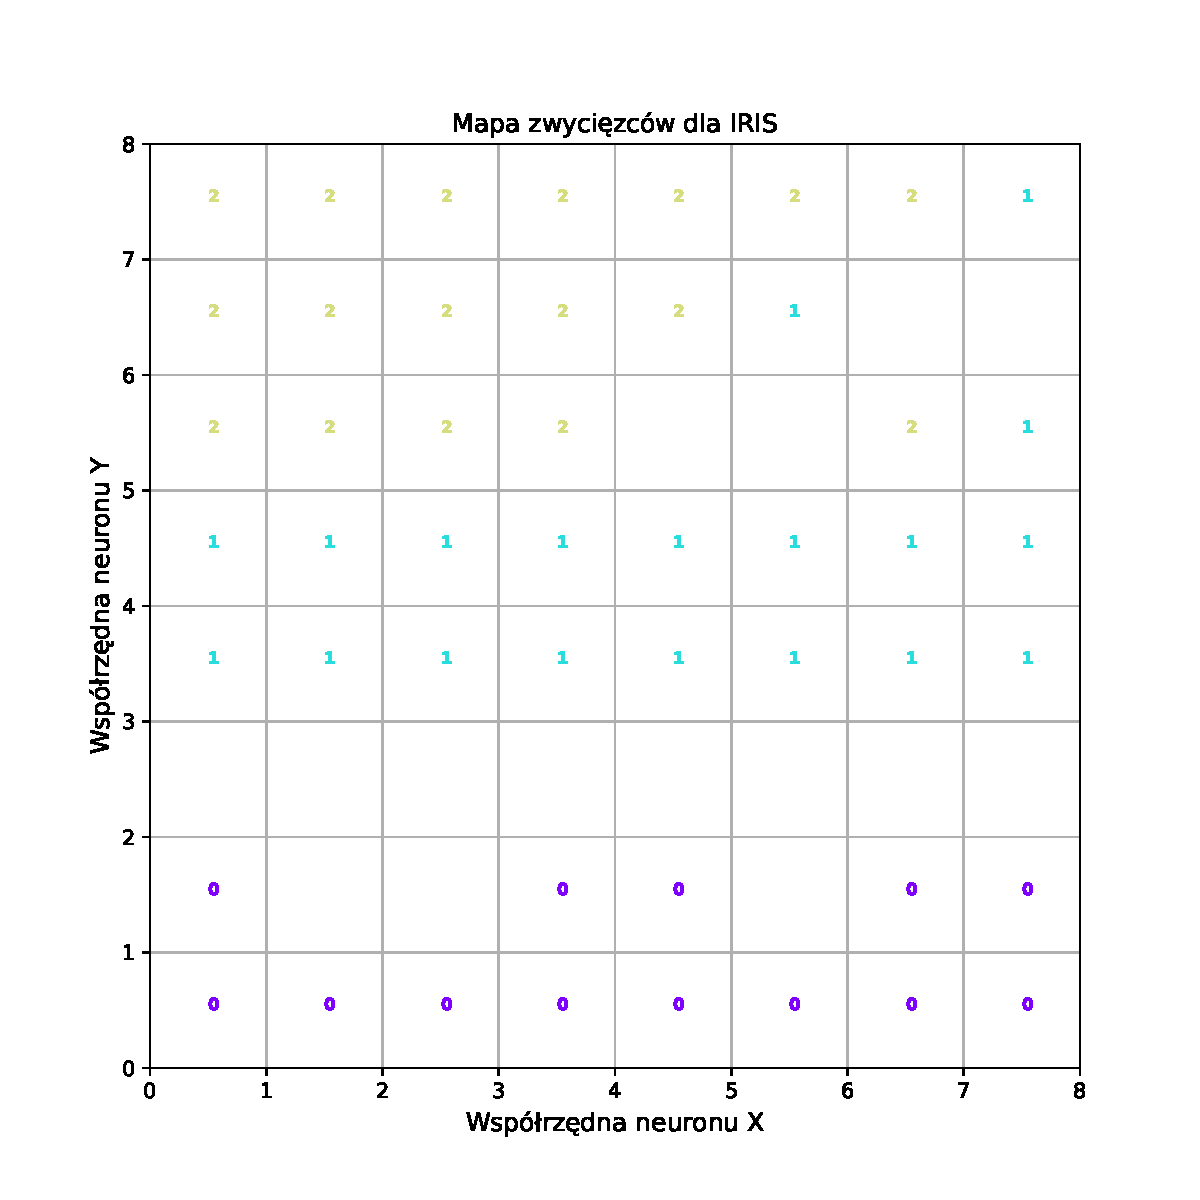
\includegraphics[width=0.8\textwidth]{./img/Iris_best.pdf}
    \caption{Mapa zwycięzców otrzymana w wyniku testów na zbiorze  IRIS}
    \label{fig:Iris_best}
\end{figure}

%PATOLOGIE SEKCJA
\section{Badania na zbiorze Cardiotocography}\label{Patologie_sekcja}
Zbiór danych Cardiotocography zawiera dane medyczne pozyskane z badań kardiotokografi (CTG), analizujących akcję serca płodu ludzkiego. Informacje umieszczone w tym zbiorze zostały udostępnione przez Instytut Położnictwa i Ginekologii Uniwersytetu Medycznego w Porto w Portugalii \cite{Patologie}. Zbiór danych zawiera 2126 próbek, każda z 21 cechami, takimi jak liczba uderzeń serca na minutę, czy liczba ruchów płodu. Oprócz cech każda z wartości ma przypisaną jedną z trzech etykiet, przypisanych przez lekarzy położników:
\begin{itemize}
    \item 1 - \textbf{Normalny (ang. Normal)}: oznaczający brak problemów zdrowotnych, liczność podzbioru danych wynosi 1655,
    \item 2 - \textbf{Podejrzany (ang. Suspect)}: wymagający dalszej obserwacji, liczność podzbioru danych wynosi 295,
    \item 3 - \textbf{Patologiczny (ang. Pathologic)}: wskazujący na możliwe komplikacje, liczność podzbioru danych wynosi 176.
\end{itemize}

Z punktu widzenia analizy danych zbiór uczący zawiera niewiele klas, za to dane posiadają wiele wymiarów. Należy również uwzględnić, że jedna z tych klas jest zdecydowanie dominująca. Wyboru dokonano zarówno ze względu na praktyczną możliwość wykorzystania sieci SOM jako narzędzia wspomagającego pracę w tak istotnej dziedzinie jak medycyna, jak i przez czysto techniczną potrzebę zbadania możliwości wykorzystania sieci przy analizie wielowymiarowych danych z niewielką liczbę klas, przy bardzo nierównomiernym rozkładzie liczby danych na klasę. 

Do tworzenia modeli wykorzystano siatkę 14 na 14 neuronów, z początkowym promieniem równym 7, a  początkową wartością współczynnika uczenia równą 0.4. Wykorzystano funkcję wykładniczą dla zmiany wartości promienia sąsiedztwa oraz funkcję wymierną dla zmiany wartości współczynnika uczenia. Ze względu na liczność zbioru danych uczących, każda z sieci była trenowana przez 1000 epok.

Wartości uzyskanych błędów kwantyzacji i błędów topograficznych przedstawione zostały w tabeli \ref{patologie_tabela}
%Tabela patologie
\begin{table}[h]
\centering
\caption{Wartości błędów topograficznych i kwantyzacji  z testów na zbiorze Cardiotocography}
\label{patologie_tabela}
\begin{tabular}{|l|l|l|l|l|l|}
\hline
\textbf{\begin{tabular}[c]{@{}l@{}}funkcja\\ sasiedztwa\end{tabular}} & \textbf{Rodzaj błędu} & \(\textbf{hex}_{ncp}\) & \(\textbf{rect}_{ncp}\) & \(\textbf{hex}_{cp}\) & \(\textbf{rect}_{cp}\) \\ \hline
\multirow{2}{*}{\textbf{Gaussa}}                                      & błąd kwantyzacji      & 0.3482                 & 0.3522                  & 0.3460                & 0.3390                 \\ \cline{2-2}
                                                                      & błąd topograficzny    & 0.0281                 & 0.0962                  & 0.0398                & 0.1032                 \\ \hline
\multirow{2}{*}{\textbf{trójkątna}}                                   & błąd kwantyzacji      & 0.3242                 & 0.3222                  & 0.3474                & 0.3141                 \\ \cline{2-2}
                                                                      & błąd topograficzny    & 0.2159                 & 0.3556                  & 0.2523                & 0.3638                 \\ \hline
\multirow{2}{*}{\textbf{prostokątna}}                                     & błąd kwantyzacji      & 0.3661                 & 0.3620                  & 0.3564                & 0.3472                 \\ \cline{2-2}
                                                                      & błąd topograficzny    & 0.0680                 & 0.1737                  & 0.0986                & 0.1807                 \\ \hline
\multirow{2}{*}{\textbf{eksponencjalna}}                              & błąd kwantyzacji      & 0.3524                 & 0.3496                  & 0.3560                & 0.3470                 \\ \cline{2-2}
                                                                      & błąd topograficzny    & 0.0728                 & 0.1995                  & 0.0751                & 0.2078                 \\ \hline
\end{tabular}
\end{table}



\subsection{Wnioski z badań na zbiorze Cardiotocography}
Z uwagi na ilość wymiarów danych maksymalny błąd kwantyzacji, wyznaczony za pomocą zależności~\ref{maksymalny_blad_kwantyzacji}, przyjmuje wartość \(\sqrt{21} \approx 4.58\). 

Najmniejszy z otrzymanych błędów kwantyzacji, wynoszący 0.3141, osiągnięto przy zastosowaniu funkcji trójkątnej, wraz funkcją zmiany promienia przyjmującą wartości całkowite oraz prostokątna topologią sieci. Stanowi on \(7.034\%\) wartości maksymalnej. W przypadku tego badania błąd topograficzny ma jednak bardzo wysoką wartość, co skutkowało niepoprawnym grupowaniem na mapie zwycięzców. 
\\Zastosowanie funkcji trójkątnej, w ogólności, przekładało się na niskie wartości błędów kwantyzacji, przy równoczesnym wzroście wartości błędów topograficznych, w stosunku do innych zastosowanych metod. Było to szczególnie widoczne przy stosowaniu funkcji zmiany promienia z całkowitymi wartościami. Tak wysokie błędy topograficzne dyskwalifikują możliwość zastosowania zaproponowanej funkcji trójkątnej do użycia na zbiorze Cardiotocography. 

Zarówno zastosowanie funkcji progowej jak i eksponencjalnej przyniosło podobne rezultaty. Błędy topograficzne miały mniejszą wartość w odniesieniu do funkcji trójkątnej, przy lekko większej wartości błędów kwantyzacji. Mapy zwycięzców jednak cechowały się dużo lepszym grupowaniem, choć nie aż tak dobrym, jak dla funkcji Gaussa. W przypadku tych funkcji można stwierdzić, że wybór całkowitego promienia spowodował większe wartości błędów kwantyzacji i topograficznych. 

Zastosowanie funkcji Gaussa okazało się najtrafniejszym wyborem, w kontekście jednoczesnego zmniejszania błędu kwantyzacji i topograficznego. Mapa zwycięzców dla funkcji Gaussa z zastosowaniem funkcji z niecałkowitą zmianą promienia oraz topologią heksagonalną przedstawiona została na rysunku \ref{fig:Fetal_best}. Wybór funkcji Gaussa przełożył się na najbardziej precyzyjne grupowanie danych, w odniesieniu do innych zastosowanych funkcji.

W badaniu na zbiorze Cardiotocography zastosowanie topologii heksagonalnej prowadziło do znacznego zmniejszania błędu topograficznego, niekiedy kosztem minimalnego wzrostu błędu kwantyzacji. Zauważono również, że analiza wartości błędu topograficznego jest bardziej miarodajna w kontekście interpretacji grupowania za pomocą  mapy zwycięzców, niż wartość błędu kwantyzacji. Niższy błąd topograficzny skutkuje zdecydowanie lepszym grupowaniem, nawet w przypadku większego błędu kwantyzacji.

W przeprowadzonym badaniu wybór niecałkowitego promienia wpłynął przede wszystkim na wartość błędu topograficznego, znacząco zmniejszając jego wartość w porównaniu do konfiguracji z promieniem przyjmującym wyłącznie wartości całkowite. 

Grupowanie pokazane na rysunku \ref{fig:Fetal_best} daje zadowalające wyniki, choć nie bardzo dobre. Zdarzają się etykiety danych "podejrzanych"\ pośród wyników "normalnych". Również jedna z danych opatrzona etykietą "patologiczne"\ została zaklasyfikowana łącznie z danymi "podejrzanymi". Wyniki te sugerują, że sieć SOM z algorytmem WTM może być użyteczna w klasyfikacji tego typu danych, jednak dla pełniejszej skuteczności konieczne byłoby zastosowanie innej techniki klasyfikacyjnej, lepiej dostosowanej do specyfiki danych. Stosowanie wyłącznie sieci Kohonena  może być narzędziem jedynie wspomagającym analizę i  klasyfikacje danego przypadku. Przy podjęciu ostatecznej decyzji kluczowa powinna być jednak ocena specjalisty, szczególnie w tak wrażliwej dziedzinie, jak klasyfikacja danych medycznych.
\begin{figure}[h]
    \centering
    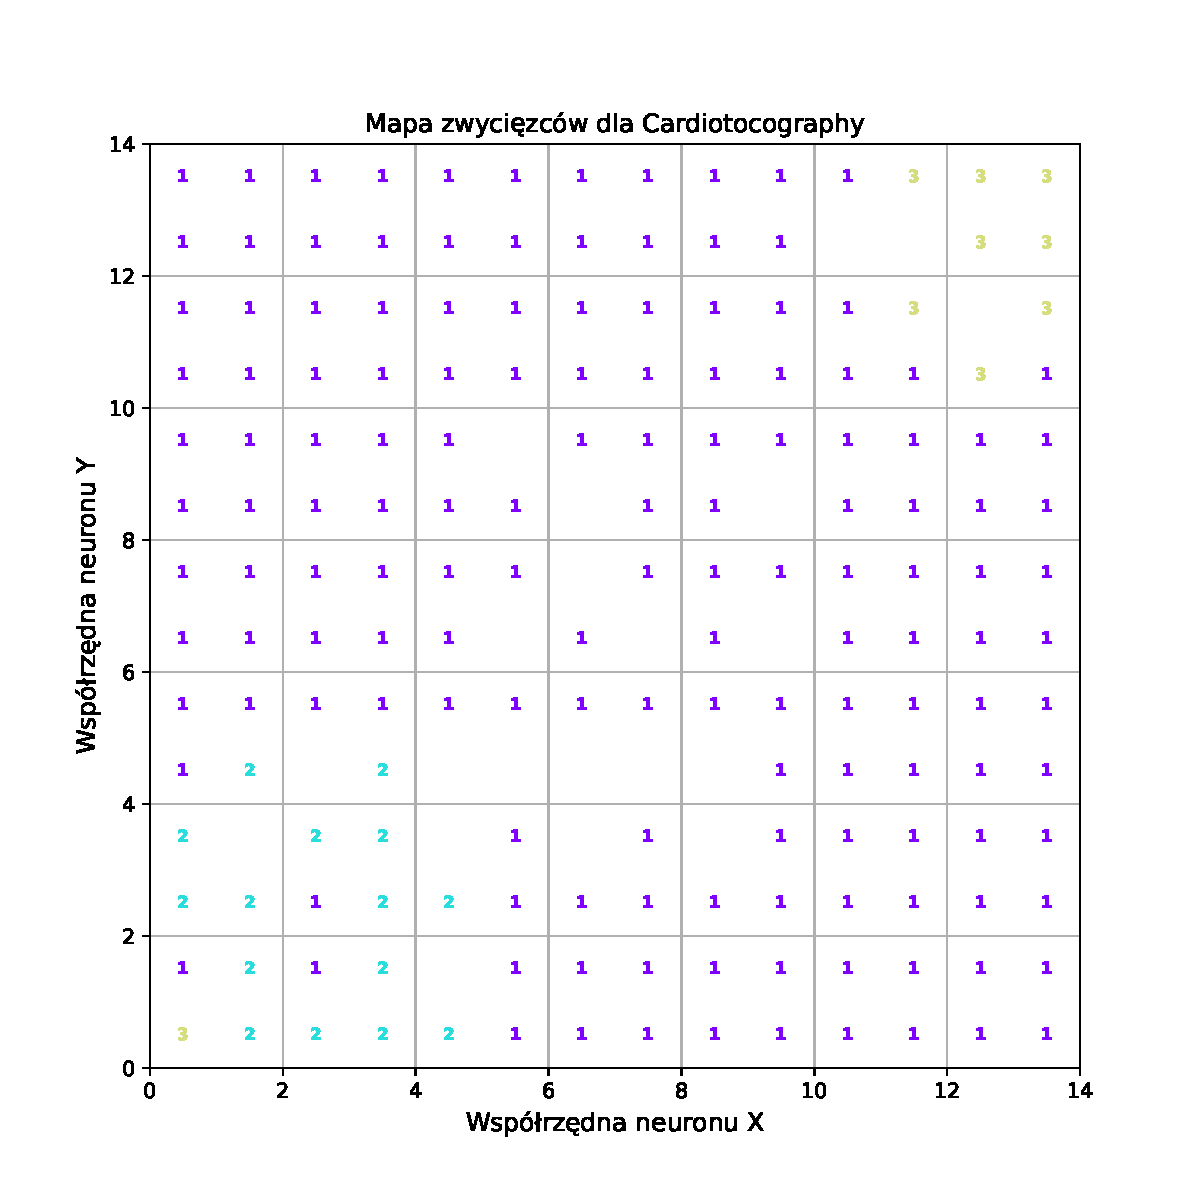
\includegraphics[width=0.8\textwidth]{./img/Fetal_best}
    \caption{Mapa zwycięzców otrzymana w wyniku testów na zbiorze Cardiotocography}
    \label{fig:Fetal_best}
\end{figure}
%MNIST wyniki
\section{Badania na zbiorze MNIST}\label{MNIST_sekcja}
Badaniami objęto również zbior MNIST (ang. "\textit{Modified National Institute of Standards and Technology dataset}", tłumaczenie: "zmodyfikowany zbiór danych Narodowego Instytutu Standardów i Technologii") \cite{MNIST}. Został on stworzony w 1998 roku, jako zmodyfikowana wersja zbioru NIST. Jest to jeden z najbardziej popularnych zbiorów danych przeznaczonych do klasyfikacji i klasteryzacji. Zbiór ten zawiera 70 000 obrazów ręcznie pisanych cyfr w skali szarości, o rozmiarze 28x28 pikseli. Każdy obraz przypisany jest do jednej z dziesięciu klas, odpowiadających cyfrom od 0 do 9. W tym zbiorze etykiety reprezentują wartości numeryczne przypisane do każdego obrazu, jednoznacznie identyfikując przedstawioną na nim cyfrę (od 0 do 9). W wyniku wykorzystania skali szarości,  po spłaszczeniu obrazu do jednowymiarowego wektora każda z danych ma 784 wymiary. 

Decyzja o przeprowadzeniu badań na tym zbiorze wynikała z konieczności zbadania możliwości stosowania sieci SOM w zbiorach danych z dużą liczbą wzorców wejściowych, w których każdy wektor wejściowy ma wiele cech. Rozłożenie liczebności w klasach jest równomierne, jednak istnieje możliwość błędnej klasyfikacji danych, ze względu na ich stopień podobieństwa. Przy tak wysokiej liczbie cech istnieje bardzo duże prawdopodobieństwo błędnej klasyfikacji.
Może to wynikać między innymi z różnic w stylach pisma i podobieństwa niektórych cyfr (np. "3"\ i "8"\ lub "4"\ i "9"). Badanie może również pokazać zdolności do zachowywania topologii wielowymiarowych danych wejściowych w tak dużym i zróżnicowanym zbiorze danych. W taki przypadku oczekuje się, że na mapie zwycięzców etykiety liczbowe danych podobnych do siebie wizualnie będą znajdowały się w niedalekiej odległości (na przykład klasa z etykietą "2"\ powinna być zlokalizowana w pobliżu klasy z etykietą "8").

Trening sieci przeprowadzono dla siatek 30 na 30 neuronów, z początkowym promieniem równym 15 i początkową wartością współczynnika uczenia równą 0.5. Wykorzystano funkcję dążącą do jedności dla zmiany wartości promienia \ref{eq:decay_to_one} oraz funkcję wymierną dla zmiany wartości współczynnika uczenia \ref{eq:exponential_decay}. Każda sieć była trenowana przez 200 epok. Z uwagi na wysoką liczbę neuronów w sieci przy procesie treningu skorzystano z zaimplementowanej możliwości obliczeń używających tensorów, wykorzystując przy tym procesor graficzny.

Wyniki otrzymanych błędów kwantyzacji i topograficznych przedstawiono w tabeli \ref{MNIST_wyniki}.


\begin{table}[h]
\centering
\caption{Wartości błędów topograficznych i kwantyzacji  z testów na zbiorze MNIST}
\label{MNIST_wyniki}
\begin{tabular}{|l|l|c|c|c|c|}
\hline
\textbf{\begin{tabular}[c]{@{}l@{}}funkcja\\ sasiedztwa\end{tabular}} & \textbf{Rodzaj błędu} & \multicolumn{1}{l|}{\(\textbf{hex}_{ncp}\)} & \multicolumn{1}{l|}{\(\textbf{rect}_{ncp}\)} & \multicolumn{1}{l|}{\(\textbf{hex}_{cp}\)} & \multicolumn{1}{l|}{\(\textbf{rect}_{cp}\)} \\ \hline
\multirow{2}{*}{\textbf{gaussa}}                                      & błąd kwantyzacji      & 4.890                                       & 4.953                                        & 4.906                                      & 5.022                                       \\ \cline{2-2}
                                                                      & błąd topograficzny    & 0.039                                       & 0.113                                        & 0.064                                      & 0.127                                       \\ \hline
\multirow{2}{*}{\textbf{trójkątna}}                                   & błąd kwantyzacji      & 4.913                                       & 4.954                                        & 4.913                                      & 5.236                                       \\ \cline{2-2}
                                                                      & błąd topograficzny    & 0.053                                       & 0.121                                        & 0.067                                      & 0.149                                      \\ \hline
\multirow{2}{*}{\textbf{prostokątna}}                                     & błąd kwantyzacji      & 5.110                                       & 5.221                                        & 4.923                                      & 5.334                                       \\ \cline{2-2}
                                                                      & błąd topograficzny    & 0.114                                       & 0.242                                       & 0.151                                      & 0.352                                       \\ \hline
\multirow{2}{*}{\textbf{eksponencjalna}}                              & błąd kwantyzacji      & 4.952                                       & 4.982                                        & 4.915                                      & 5.312                                       \\ \cline{2-2}
                                                                      & błąd topograficzny    & 0.073                                       & 0.125                                        & 0.062                                      & 0.144                                       \\ \hline
\end{tabular}
\end{table}
\subsection{Wnioski z badań na zbiorze MNIST}
Dla zbioru MNIST, z uwagi na dużą liczbę wymiarów wektorów wejściowych, maksymalny błąd kwantyzacji, wyznaczony za pomocą zależności \ref{maksymalny_blad_kwantyzacji}, przyjmuje wartość \(\sqrt{784} = 28\). 
Średni błąd kwantyzacji dla wszystkich badań wyniósł 5.033, co stanowi \(17.9\%\) wartości maksymalnej. Jest to wynik relatywnie wysoki, jednak spodziewany, ze względu na dużą ilość danych uczących, z wieloma wymiarami. Miara ta jednak nie skreśla zastosowania sieci SOM przy klasyfikowaniu takich obrazów, jak te w zbiorze MNIST.
Wartości błędów kwantyzacji nie różniły się znacząco miedzy sobą, niezależnie od zastosowanej funkcji sąsiedztwa, jednak błędy topograficzne miały zupełnie inne wartości, w zależności od zastosowanej funkcji sąsiedztwa.

Zastosowanie funkcja progowej doprowadziło do największych błędów topograficznych. Lepsze rezultaty osiągnięto przy niecałkowitej zmianie promienia sąsiedztwa, jednak nie są to na tyle niskie wartości, aby umożliwić poprawną klasyfikację obrazów przedstawiających liczby. Również mapy zwycięzców dla tej funkcji cechowały się niepoprawnym grupowaniem i zupełnym niezachowywaniem relacji w danych wejściowych.

Badania z wykorzystaniem funkcji trójkątnej i funkcji eksponencjalnej skutkowały bardzo zbliżonymi wartościami błędów, zarówno kwantyzacji jak i topograficznych. Z tych dwóch podejść jednak uzyskano nieznacznie lepsze rezultaty na mapie zwycięzców, wykorzystując funkcję trójkątną. Podobnie jak przy zastosowaniu funkcji progowej, w tych wypadkach również lepiej sprawdzały się topologie heksagonalne, wraz z niecałkowitą zmianą promienia. Mapy zwycięzców dla przypadków stosowania funkcji trójkątnej były w ogólności bardziej precyzyjne niż te stworzone za pomocą sieci trenowanych funkcją eksponencjalną. Mapy te były bardzo zbliżone do najlepszych wyników, uzyskanych za pomocą funkcji Gaussa.

Najniższe wartości błędów kwantyzacji i topograficznych uzyskano dla zastosowania funkcji Gaussa. Najlepsze grupowanie uzyskano, stosując w funkcje zmiany promienia przyjmującą wartości niecałkowite oraz topologie heksagonalną. Mapę zwycięzców dla tego przypadku przedstawiono na \ref{fig:MNIST_best}. W innych przypadkach osiągano zbliżone wartości błędów kwantyzacji, jednak błędy topograficzne istotnie się różniły. Osiągnięto lepsze rezultaty stosując topologię heksagonalną. 

Z badań przeprowadzonych na zbiorze MNIST można wyciągnąć pewne wnioski. Stosowanie niecałkowitych wartości promienia prowadzi do zmniejszenia wartości błędów topograficznych przy przypisywaniu danych z tego zbioru do klas. Jest to niezależne od zastosowanej funkcji sąsiedztwa. Dodatkowo, najlepsze rezultaty osiągnięto za pomocą funkcji Gaussa, co jest zgodne z trendami badań w literaturze \cite{Kolasa_artykul,DeepSOM}. Niewiele gorsze rezultaty uzyskano za pomocą funkcji trójkątnej i eksponencjalnej, przy czym pierwsza z nich dała nieznacznie lepsze rezultaty. Funkcja prostokątna nie umożliwiła poprawnego przypisania do klas danych ze zbioru MNIST.
\\ W przypadku rozważania wpływu topologii sieci na wartość błędów oraz na jakość mapy zwycięzców, można stwierdzić, że zastosowanie topologii heksagonalnej poprawiło efekty wszystkich miar. Może być to powiązane ze specyficzną strukturą danych ze zbioru MNIST.

Przedstawiona na rysunku \ref{fig:MNIST_best} mapa zwycięzców poprawnie odwzorowuje strukturę danych wejściowych, wykazując widoczne lokalne skupiska odpowiadające określonym klasom, takim jak 3, 7, 2 czy 0. Niemniej jednak, w niektórych obszarach pojawia się mieszanie klas lub brak jednoznacznego przypisania. Topologia danych została zachowana w znacznym stopniu, choć można również zauważyć błędy w przypisaniu. Rezultaty te oznaczają, że stosowanie jedynie sieci SOM, bez innych narzędzi analizy danych, nie gwarantuje idealnego przypisywania do klas tak złożone dane  jak obrazy rozmiaru 28x28. 
 
\begin{figure}[h]
    \centering
    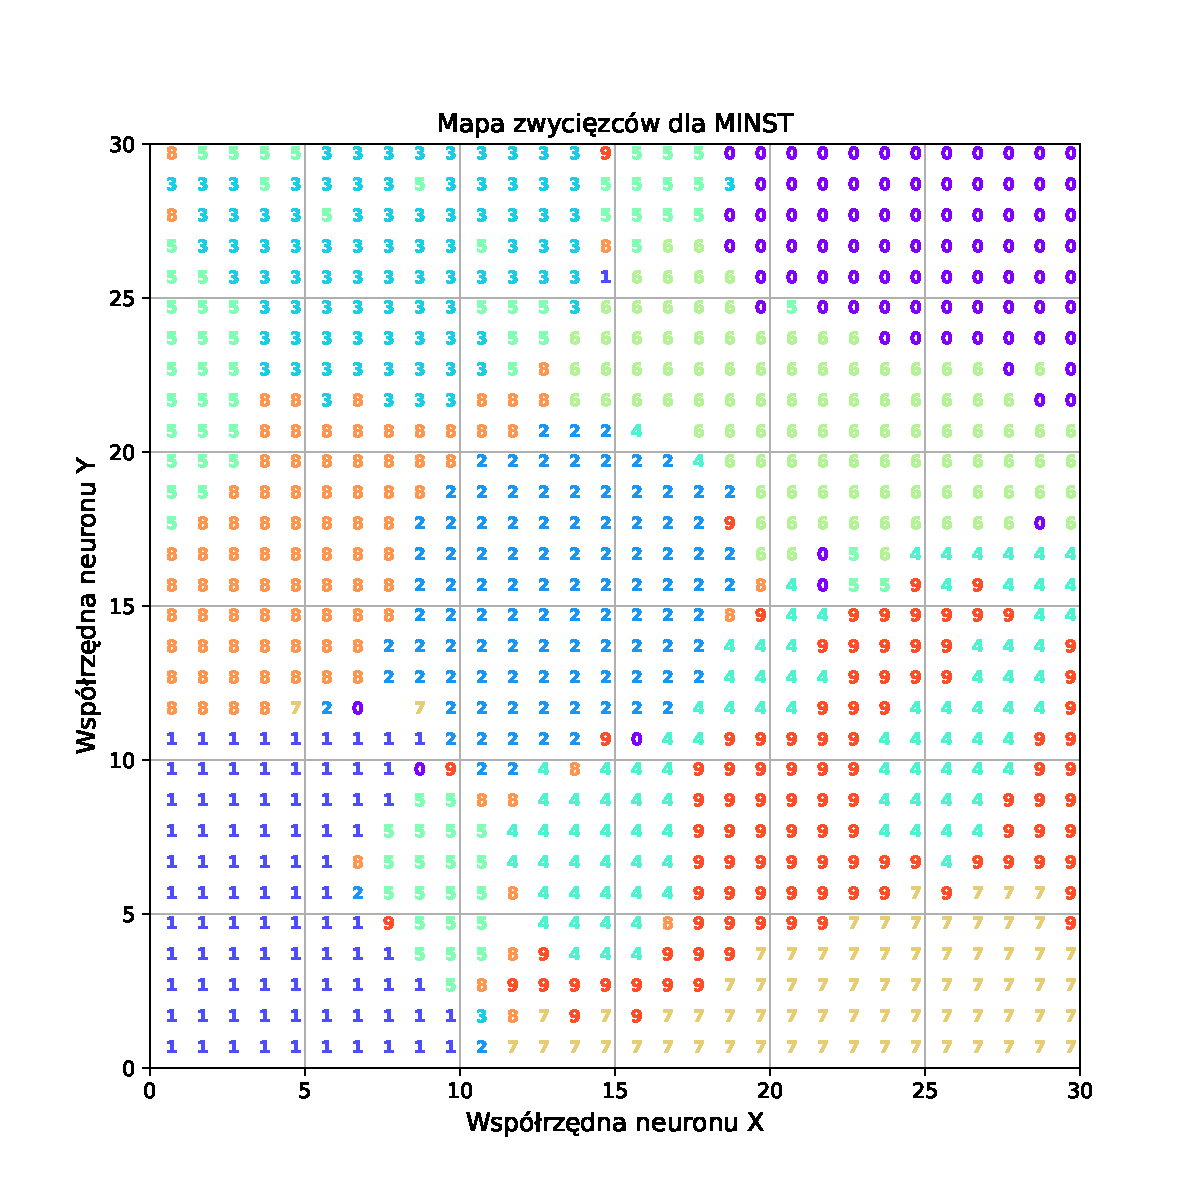
\includegraphics[width=0.8\textwidth]{./img/MNIST_best.pdf}
    \caption{Mapa zwycięzców otrzymana w wyniku testów na zbiorze MNIST}
    \label{fig:MNIST_best}
\end{figure}

